%%%%%%%%%%%%%%%%%%%%%%%%%%%%%%%%%%%%

\section{Difference of two means}

%%%%%%%%%%%%%%%%%%%%%%%%%%%%%%%%%%%%

\begin{frame}
\frametitle{Diamonds}

\begin{itemize}

\item Weights of diamonds are measured in carats. 

\item 1 carat = 100 points, 0.99 carats = 99 points, etc.

\item The difference between the size of a 0.99 carat diamond and a 1 carat diamond is undetectable to the naked human eye, but does the price of a 1 carat diamond tend to be higher than the price of a 0.99 diamond?

\item We are going to test to see if there is a difference between the average prices of 0.99 and 1 carat diamonds.

\item In order to be able to compare equivalent units, we divide the prices of 0.99 carat diamonds by 99 and 1 carat diamonds by 100, and compare the average point prices.

\end{itemize}

\hfill 
\includegraphics[width=0.3\textwidth]{5-3_diff_two_mean/figures/diamonds/diamond}

\end{frame}

%%%%%%%%%%%%%%%%%%%%%%%%%%%%%%%%%%%

\begin{frame}[fragile]
\frametitle{Data}

\begin{center}
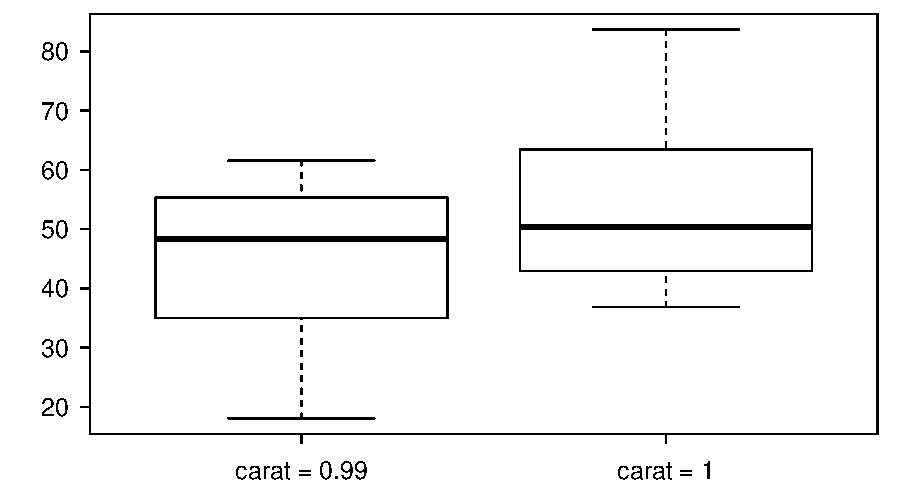
\includegraphics[width=0.7\textwidth]{5-3_diff_two_mean/figures/diamonds/diamondBox}
\end{center}

{\small
\begin{center}
\begin{tabular}{l | c | c}
		& {\footnotesize \hl{0.99 carat}} &  {\footnotesize \hl{1 carat}}  \\
		& pt99	& pt100 \\
\hline
$\bar{x}$	& 44.50		& 53.43 \\
$s$		& 13.32		& 12.22 \\
$n$		& 23			& 30
\end{tabular}
\end{center}
}

\vfill

\rule{2.5cm}{0.25pt} \\
{\tiny These data are a random sample from the \texttt{diamonds} data set in \texttt{ggplot2} R package.}

\end{frame}

%%%%%%%%%%%%%%%%%%%%%%%%%%%%%%%%%%%

\begin{frame}
\frametitle{Parameter and point estimate}

\begin{itemize}

\item \hl{Parameter of interest:} Average difference between the point prices of \orange{all} 0.99 carat and 1 carat diamonds.
\[ \mu_{pt99} - \mu_{pt100} \]

$\:$ \\

\pause

\item \hl{Point estimate:} Average difference between the point prices of \orange{sampled}  0.99 carat and 1 carat diamonds.
\[ \bar{x}_{pt99} - \bar{x}_{pt100} \]

\end{itemize}

\end{frame}

%%%%%%%%%%%%%%%%%%%%%%%%%%%%%%%%%%%

\begin{frame}
\frametitle{Hypotheses}

\pq{Which of the following is the correct set of hypotheses for testing if the average point price of 1 carat diamonds ($_{pt100}$) is higher than the average point price of 0.99 carat diamonds ($_{pt99}$)?}

\begin{enumerate}[(a)]

\item  \mathhl{H_0:} $\mu_{pt99} = \mu_{pt100}$ \\
\mathhl{H_A:} $\mu_{pt99} \ne \mu_{pt100}$

\item  \mathhl{H_0:} $\mu_{pt99} = \mu_{pt100}$ \\
\mathhl{H_A:} $\mu_{pt99} > \mu_{pt100}$

\solnMult{  \mathhl{H_0:} $\mu_{pt99} = \mu_{pt100}$ \\
\mathhl{H_A:} $\mu_{pt99} < \mu_{pt100}$ }

\item  \mathhl{H_0:} $\bar{x}_{pt99} = \bar{x}_{pt100}$ \\
\mathhl{H_A:} $\bar{x}_{pt99} < \bar{x}_{pt100}$

\end{enumerate}

\end{frame}

%%%%%%%%%%%%%%%%%%%%%%%%%%%%%%%%%%%

\begin{frame}
\frametitle{Conditions}

\pq{Which of the following does \underline{not} need to be satisfied in order to conduct this hypothesis test using theoretical methods?}

\begin{enumerate}[(a)]

\item Point price of one 0.99 carat diamond in the sample should be independent of another, and the point price of one 1 carat diamond should independent of another as well.

\item Point prices of 0.99 carat and 1 carat diamonds in the sample should be independent.

\item Distributions of point prices of 0.99 and 1 carat diamonds should not be extremely skewed.

\solnMult{Both sample sizes should be at least 30.}

\end{enumerate}

\end{frame}

%%%%%%%%%%%%%%%%%%%%%%%%%%%%%%%%%%%%

\subsection{Sampling distribution for the difference of two means}

%%%%%%%%%%%%%%%%%%%%%%%%%%%%%%%%%%%%

\begin{frame}
\frametitle{Test statistic}

\formula{Test statistic for inference on the difference of two small sample means}
{The test statistic for inference on the difference of two means where $\sigma_1$ and $\sigma_2$ are unknown is the $T$ statistic.
\[ T_{df} = \frac{\text{point estimate} - \text{null value}}{SE} \]
where 
\[ SE = \sqrt{ \frac{s_1^2}{n_1} + \frac{s_2^2}{n_2} } \qquad \text{ and } \qquad df = min(n_1 - 1, n_2 - 1) \]
}

\Note{The calculation of the $df$ is actually much more complicated. For simplicity we'll use the above formula to \underline{estimate} the true $df$ when conducting the analysis by hand.}

\end{frame}

%%%%%%%%%%%%%%%%%%%%%%%%%%%%%%%%%%%%

\subsection{Hypothesis testing for the difference of two means}

%%%%%%%%%%%%%%%%%%%%%%%%%%%%%%%%%%%%

\begin{frame}
\frametitle{Test statistic (cont.)}

{\small
\begin{center}
\begin{tabular}{l | c | c}
		& {\footnotesize \hl{0.99 carat}} &  {\footnotesize \hl{1 carat}}  \\
		& pt99	& pt100 \\
\hline
$\bar{x}$	& 44.50		& 53.43 \\
$s$		& 13.32		& 12.22 \\
$n$		& 23			& 30
\end{tabular}
\end{center}
}

\hl{in context...}

\pause

{\small
\begin{eqnarray*}
T &=& \frac{\text{point estimate} - \text{null value} }{SE} \\
\pause
&=& \frac{(44.50 - 53.43) - 0}{ \sqrt{\frac{13.32^2}{23} + \frac{12.22^2}{30} }} \\
\pause
&=& \frac{-8.93}{3.56} \\
\pause
&=& -2.508
\end{eqnarray*}
}

\end{frame}

%%%%%%%%%%%%%%%%%%%%%%%%%%%%%%%%%%%%

\begin{frame}
\frametitle{Test statistic (cont.)}

\pq{Which of the following is the correct $df$ for this hypothesis test?}

\twocol{0.3}{0.7}
{
\begin{enumerate}[(a)]
\solnMult{ 22 }
\item 23
\item 30
\item 29
\item 52
\end{enumerate}
}
{
\soln{\only<2>{
\orange{$\rightarrow df = min(n_{pt99} - 1, n_{pt100} - 1)$ \\
$= min(23 - 1, 30 - 1)$ \\
$= min(22,29) = 22$} \\
\vspace{1cm}
}}}

\end{frame}

%%%%%%%%%%%%%%%%%%%%%%%%%%%%%%%%%%%%

\begin{frame}
\frametitle{p-value}

\pq{Which of the following is the correct p-value for this hypothesis test?}

\[ T = -2.508 \qquad \only<1-2 | handout:0>{df = 22} \] 

\twocol{0.42}{0.58}
{
\begin{enumerate}[(a)]
\item between 0.005 and 0.01
\solnMult{between 0.01 and 0.025}
\item between 0.02 and 0.05
\item between 0.01 and 0.02
\end{enumerate}
}
{
\only<1>{
{\footnotesize
\begin{tabular}{r | r r  r r r}
\hline
one tail & \hspace{1.5mm}  0.100 & \hspace{1.5mm} 0.050 & \hspace{1.5mm} {0.025} & \hspace{1.5mm} {0.010} & \hspace{1.5mm} 0.005  \\
two tails & 0.200 & 0.100 & 0.050 & 0.020 & 0.010 \\
\hline
df \hfill 21  &  {  1.32} & {  1.72} & {  2.08} & {  2.52} & {  2.83}  \\ 
22  &  {  1.32} & {  1.72} & {  2.07} & {  2.51} & {  2.82}  \\ 
23  &  {  1.32} & {  1.71} & {  2.07} & {  2.50} & {  2.81}  \\ 
24  &  {  1.32} & {  1.71} & {  2.06} & {  2.49} & {  2.80}  \\ 
25  &  {  1.32} & {  1.71} & {  2.06} & {  2.49} & {  2.79}  \\ 
\hline
\end{tabular}
}
}

\only<2|handout:0>{
{\footnotesize
\begin{tabular}{r | r r  >{\columncolor[gray]{.6}[.5\tabcolsep]}r  >{\columncolor[gray]{.6}[.5\tabcolsep]}r r}
\hline
one tail & \hspace{1.5mm}  0.100 & \hspace{1.5mm} 0.050 & \hspace{1.5mm} \orange{0.025} & \hspace{1.5mm} \orange{0.010} & \hspace{1.5mm} 0.005  \\
two tails & 0.200 & 0.100 & 0.050 & 0.020 & 0.010 \\
\hline
df \hfill 21  &  {  1.32} & {  1.72} & {  2.08} & {  2.52} & {  2.83}  \\ 
  \rowcolor[gray]{.6}
22  &  {  1.32} & {  1.72} & \orange{  2.07} & \orange{  2.51} & {  2.82}  \\ 
23  &  {  1.32} & {  1.71} & {  2.07} & {  2.50} & {  2.81}  \\ 
24  &  {  1.32} & {  1.71} & {  2.06} & {  2.49} & {  2.80}  \\ 
25  &  {  1.32} & {  1.71} & {  2.06} & {  2.49} & {  2.79}  \\ 
\hline
\end{tabular}
}
}}

\end{frame}

%%%%%%%%%%%%%%%%%%%%%%%%%%%%%%%%%%%%

\begin{frame}
\frametitle{Synthesis}

\dq{What is the conclusion of the hypothesis test? How (if at all) would this conclusion change your behavior if you went diamond shopping?}


\soln{\only<2>{
\begin{itemize}
\item p-value is small so reject $H_0$. The data provide convincing evidence to suggest that the point price of 0.99 carat diamonds is lower than the point price of 1 carat diamonds.
\item Maybe buy a 0.99 carat diamond? It looks like a 1 carat, but is significantly cheaper.
\end{itemize}
}}

\end{frame}

%%%%%%%%%%%%%%%%%%%%%%%%%%%%%%%%%%%%

\subsection{Confidence intervals for the difference of two means}

%%%%%%%%%%%%%%%%%%%%%%%%%%%%%%%%%%%%

\begin{frame}
\frametitle{Equivalent confidence level}

\pq{What is the equivalent confidence level for a one-sided hypothesis test at $\alpha = 0.05$?}


\twocol{0.3}{0.7}{
\begin{enumerate}[(a)]

\solnMult{90\%}

\item 92.5\%

\item 95\%

\item 97.5\%

\end{enumerate}
}
{
\soln{\only<2>{
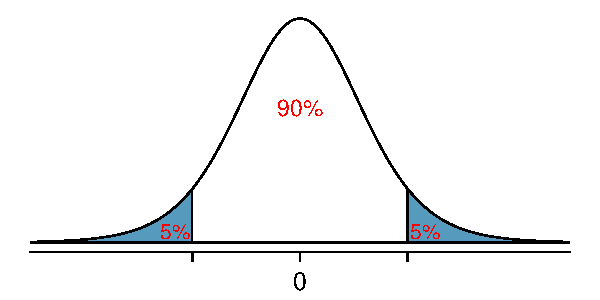
\includegraphics[width=\textwidth]{5-3_diff_two_mean/figures/middle90/middle90}
}}
}

\end{frame}

%%%%%%%%%%%%%%%%%%%%%%%%%%%%%%%%%%%%

\begin{frame}
\frametitle{Critical value}

\pq{What is the appropriate $t^\star$ for a confidence interval for the average difference between the point prices of 0.99 and 1 carat diamonds?}

\begin{enumerate}[(a)]
\item 1.32
\solnMult{1.72}
\item 2.07
\item 2.82
\end{enumerate}

\only<1>{
{\small
\begin{center}
\begin{tabular}{r | r r r r r}
\hline
one tail & \hspace{1.5mm}  0.100 & \hspace{1.5mm} {0.050} & \hspace{1.5mm} {0.025} & \hspace{1.5mm} {0.010} & \hspace{1.5mm} 0.005  \\
two tails & 0.200 & 0.100 & 0.050 & 0.020 & 0.010 \\
\hline
df \hfill 21  &  {  1.32} & {  1.72} & {  2.08} & {  2.52} & {  2.83}  \\ 
22  &  {  1.32} & {  1.72} & {  2.07} & {  2.51} & {  2.82}  \\ 
23  &  {  1.32} & {  1.71} & {  2.07} & {  2.50} & {  2.81}  \\ 
24  &  {  1.32} & {  1.71} & {  2.06} & {  2.49} & {  2.80}  \\ 
25  &  {  1.32} & {  1.71} & {  2.06} & {  2.49} & {  2.79}  \\ 
\end{tabular}
\end{center}
}}

\only<2|handout:0>{
\begin{center}
{\small
\begin{tabular}{r | r >{\columncolor[gray]{.6}[.5\tabcolsep]}r r  r r}
\hline
one tail & \hspace{1.5mm}  0.100 & \hspace{1.5mm} {0.050} & \hspace{1.5mm} {0.025} & \hspace{1.5mm} {0.010} & \hspace{1.5mm} 0.005  \\
two tails & 0.200 & \orange{0.100} & 0.050 & 0.020 & 0.010 \\
\hline
df \hfill 21  &  {  1.32} & {  1.72} & {  2.08} & {  2.52} & {  2.83}  \\ 
  \rowcolor[gray]{.6}
22  &  {  1.32} & \orange{  1.72} & {  2.07} & {  2.51} & {  2.82}  \\ 
23  &  {  1.32} & {  1.71} & {  2.07} & {  2.50} & {  2.81}  \\ 
24  &  {  1.32} & {  1.71} & {  2.06} & {  2.49} & {  2.80}  \\ 
25  &  {  1.32} & {  1.71} & {  2.06} & {  2.49} & {  2.79}  \\ 
\hline
\end{tabular}
}
\end{center}
}


\end{frame}

%%%%%%%%%%%%%%%%%%%%%%%%%%%%%%%%%%%%

\begin{frame}
\frametitle{Confidence interval}

\dq{Calculate the interval, and interpret it in context.}

\pause

\soln{
\[ \text{point estimate} \pm ME \]
\pause
\begin{eqnarray*}
(\bar{x}_{pt99} - \bar{x}_{pt1}) \pm t^\star_{df} \times SE &=& (44.50 - 53.43) \pm 1.72 \times 3.56 \\
\pause
&=& -8.93 \pm  6.12 \\
\pause
&=& (-15.05, -2.81)
\end{eqnarray*}
\pause
We are 90\% confident that the average point price of a 0.99 carat diamond is \$15.05 to \$2.81 lower than the average point price of a 1 carat diamond.
}

\end{frame}

%%%%%%%%%%%%%%%%%%%%%%%%%%%%%%%%%%%%

\subsection{Recap}

%%%%%%%%%%%%%%%%%%%%%%%%%%%%%%%%%%%%

\begin{frame}
\frametitle{Recap: Inference using difference of two small sample means}

\begin{itemize}

\item If $\sigma_1$ or $\sigma_2$ is unknown, difference between the sample means follow a $t$-distribution with $SE = \sqrt{ \frac{s_1^2}{n_1} + \frac{s_2^2}{n_1} }$.

\pause

\item Conditions: 
\begin{itemize}
\item independence within groups (often verified by a random sample, and if sampling without replacement, $n < $ 10\% of population) and between groups
\item no extreme skew in either group
\end{itemize}

\pause

\item Hypothesis testing: 
\[ T_{df} = \frac{\text{point estimate} - \text{null value}}{SE}\text{, where }df = min(n_1 - 1, n_2 - 1) \]

\pause

\item Confidence interval:
\[ \text{point estimate} \pm t_{df}^\star \times SE \]

\end{itemize}

\end{frame}

%%%%%%%%%%%%%%%%%%%%%%%%%%%%%%%%%%%